\chapter{Sprint 0 : Analyse et Spécification des besoins}
\section{Introduction}
Ce chapitre est consacré à l’analyse des besoins pour le développement du Portail de Gestion des Approbations. Nous y identifions les exigences fonctionnelles et non fonctionnelles du système, puis nous illustrons la modélisation à l’aide de diagrammes UML tels que les cas d’utilisation et le diagramme de classes.\\
Nous présentons ensuite le Backlog produit défini selon la méthodologie Scrum, avant de conclure par une présentation des principaux outils utilisés dans cette phase.
\section{Capture des besoins}
Dans cette section nous présentons les acteurs du système,les besoins fonctionnels et non
fonctionnels présents dans le projet.
\subsection{Identification des acteurs}
Notre système contient quatre acteurs ,illustrés dans la figure \ref{tab:actors}, qui sont :
\begin{itemize}
    \item \textbf{Administrateur} : Gère l’ensemble du système, incluant les utilisateurs et les configurations globales (e.g., permissions, intégrations).
    \item \textbf{Manager} : Soumet, consulte et traite les demandes (validation/rejet) des employés qu’il supervise.
    \item \textbf{RH (Ressources Humaines)} : Gère les congés, soumet, consulte et traite les demandes, tout en assurant le suivi des politiques RH.
    \item \textbf{Utilisateur} : Employé qui soumet des demandes (congés, absences) et consulte ses propres demandes et soldes de congés.
\end{itemize}
\begin{figure}[h]
\vspace*{-2cm}
    \centering
    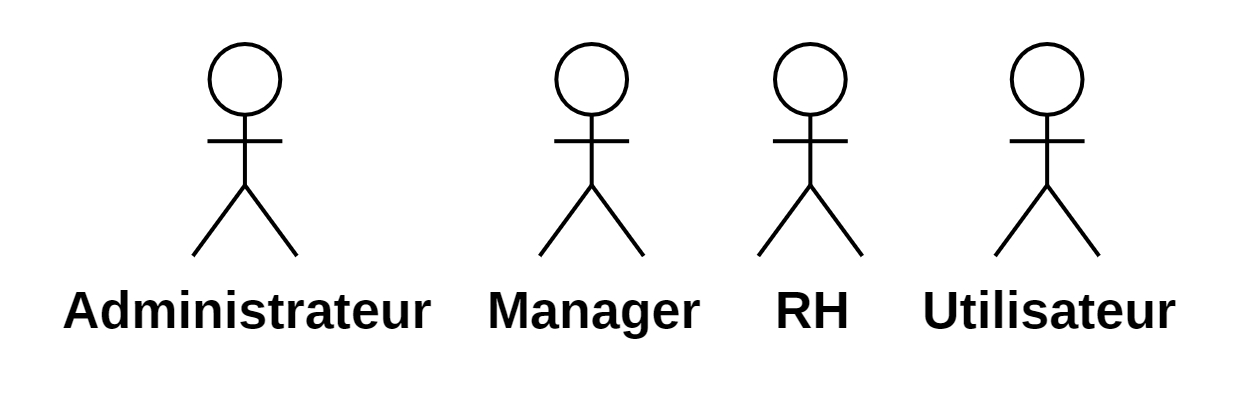
\includegraphics[width=6cm]{images/actors.jpg} 
    \caption{Les acteurs}
    \label{tab:actors}
\end{figure}
 \subsection{Identification des besoins fonctionnels}
Les besoins fonctionnels sont les interactions entre l'acteur(Une personne,un matériel ou un logiciel) et le système de manière à exploiter les fonctionnalités de ce dernier.
Notre système offre aux acteurs la possibilité de faire certaines tâches. \\
\vspace*{-0.5cm}
\begin{table}[!ht]
Le tableau \ref{tab:actors} illustre le rôle de chaque acteur dans ce système.
\begin{center}
\vspace*{-0.5cm}
\caption{tab:Les rôles des acteurs}
\begin{tabular}{ | m{4cm} | m{9cm}| } 
\hline
Administrateur &
- S'authentifier. \vskip0.05cm
- Se déconnecter. \vskip0.05cm
- Gérer les utilisateurs.\vskip0.05cm
- Consulter les processus métiers. \vskip0.05cm
- Consulter les demandes d'approbations.
 \\ 
\hline
Utilisateur &
- S’authentifier.\vskip0.05cm
- Se déconnecter.\vskip0.05cm
- Consulter ses demandes.\vskip0.05cm
- Consulter ses congés.\vskip0.05cm
- Soumettre une demande.\vskip0.05cm
- Recevoir une notifications.\vskip0.05cm
- Consulter les rapports.\vskip0.05cm
- Gérer son profil.\vskip0.05cm
- Consulter le calendrier d'équipe.\vskip0.05cm
- Consulter les membres d'équipe.\vskip0.05cm
- Consulter ses crédits.
\\
\hline
Manager / RH &
- S’authentifier.\vskip0.05cm
- Se déconnecter.\vskip0.05cm
- Consulter ses demandes.\vskip0.05cm
- Consulter ses congés.\vskip0.05cm
- Soumettre une demande.\vskip0.05cm
- Recevoir une notifications.\vskip0.05cm
- Consulter les rapports.\vskip0.05cm
- Gérer son profil.\vskip0.05cm
- Consulter le calendrier d'équipe.\vskip0.05cm
- Consulter les membres d'équipe.\vskip0.05cm
- Consulter ses crédits.\vskip0.05cm
- Consulter ses taches accomplies. \vskip0.05cm
- Traiter une Demande.
\\
\hline
\end{tabular}
\label{1}
\end{center}
\end{table}
\newpage
\subsection{Identification des cas d'utilisation}
\begin{itemize}
 \item \textbf{S'authentifier:} L'authentification est le cas d'utilisation qui permet à tous les utilisateurs (Administrateur, Utilisateur, Manager, RH) d'accéder à la plateforme. Il contient deux champs à remplir, qui sont le nom d'utilisateur et le mot de passe, et un bouton de validation pour accéder aux fonctionnalités de la plateforme en cas de succès de l'authentification.
 
 \item \textbf{Se déconnecter:} Les utilisateurs (Administrateur, Utilisateur, Manager, RH) peuvent se déconnecter du système en cliquant sur le bouton "Déconnexion". Le système vérifie l'existence et la conformité des coordonnées de l'utilisateur avant de le quitter.

 \item \textbf{Gérer les utilisateurs:} À travers ce cas d'utilisation, l'Administrateur est le seul à avoir le droit de gérer les utilisateurs de la plateforme, en incluant l'ajout, la consultation, la modification et la suppression des utilisateurs

 \item \textbf{Consulter les processus métiers:} L'Administrateur a la possibilité de consulter les différents processus métiers définis dans le système pour mieux comprendre les opérations internes et leur suivi.

 \item \textbf{Consulter les demandes d'approbation:} L'Administrateur peut accéder aux demandes d'approbation soumises pour les consulter.

 \item \textbf{Consulter ses demandes:} Les Utilisateurs, les Managers et les RH peuvent consulter l'historique de leurs demandes dans la plateforme.

 \item \textbf{Consulter ses congés:} Les utilisateurs, les Managers et les RH peuvent consulter la liste de leurs congés, passés et à venir, ainsi que leur solde restant.

 \item \textbf{Soumettre une demande:} Les Utilisateurs, les Managers et les RH peuvent soumettre une nouvelle demande via la plateforme. Cette demande peut concerner des congés, des absences ou d'autres requêtes spécifiques.

 \item \textbf{Recevoir une notification:} Ce cas permet aux Utilisateurs, Managers et aux RH de recevoir des notifications concernant les actions importantes, comme la validation d’une demande, ou des rappels de tâches.

 \item \textbf{Consulter les rapports:} Les Utilisateurs, les Managers et les RH peuvent consulter les rapports concernant leurs activités, comme les demandes soumises, les congés, les tâches accomplies, etc.

 \item \textbf{Gérer son profil:} Ce cas permet à chaque acteur (Utilisateur, Manager, RH) de gérer son profil personnel en modifiant ses informations comme son mot de passe, son adresse e-mail, etc.

 \item \textbf{Consulter le calendrier d'équipe:} Ce cas permet à l'Utilisateur, au Manager et au RH de consulter le calendrier de leur équipe, afin de voir les absences, les congés et les événements à venir.
\newpage
 \item \textbf{Consulter les membres de l'équipe:} Les Utilisateurs, les Managers et les RH peuvent consulter la liste des membres de leur équipe, leurs informations et les tâches qui leur sont attribuées.\\

 \item \textbf{Consulter ses crédits:} Ce cas permet aux Utilisateurs, aux Managers et aux RH de consulter le solde de leurs crédits de congé ou autres types de crédits sur la plateforme.

 \item \textbf{Consulter ses tâches accomplies:} Les Managers et les RH peuvent consulter les tâches accomplies par ses subordonnés, pour le suivi des activités et des performances.

 \item \textbf{Traiter une demande:} Le Manager  et l'RH sont en charge de traiter les demandes soumises, en les validant ou en les rejetant, selon les critères définis dans la plateforme.
\end{itemize}
\subsection{Identification des besoins non fonctionnels}

Les besoins non fonctionnels décrivent les contraintes et les exigences de qualité que doit respecter le système. Ils garantissent la performance, la fiabilité et la sécurité de l'application. Voici les principaux besoins non fonctionnels identifiés pour notre projet :

\begin{itemize}
    \item \textbf{Performance :} Le système doit offrir une bonne réactivité, avec un temps de réponse inférieur à 2 secondes pour l'affichage des principales fonctionnalités. Il doit également supporter un nombre élevé de connexions simultanées sans dégradation notable des performances.
    
    \item \textbf{Sécurité :} Le système doit garantir la confidentialité, l’intégrité et la disponibilité des données. L’authentification des utilisateurs doit être sécurisée, et les accès doivent être strictement contrôlés selon le rôle de chaque utilisateur.
    
    \item \textbf{Fiabilité :} Le système doit être capable de fonctionner de manière continue sans erreurs critiques, avec un taux de disponibilité supérieur à 99.5\%.

    \item \textbf{Scalabilité :} Le système doit pouvoir évoluer facilement pour prendre en charge un plus grand nombre d’utilisateurs ou de données sans refonte majeure de l’architecture.
    
    \item \textbf{Traçabilité :} Le système doit enregistrer les actions importantes effectuées par les utilisateurs (audit logs) pour permettre un suivi en cas d’incident ou d’investigation.
\end{itemize}
\newpage
\section{Diagramme de cas d'utilisation globale}
Le diagramme de cas d'utilisation globale illustré dans la figure \ref{usecaseDiagram} consiste à décrire les fonctions fondamentales et identifie , également la relation et les interactions entre le système et ses acteurs.
\begin{figure}[H]
\begin{adjustwidth}{-2.7cm}{-2cm} % reduce left and right margins locally
\centering
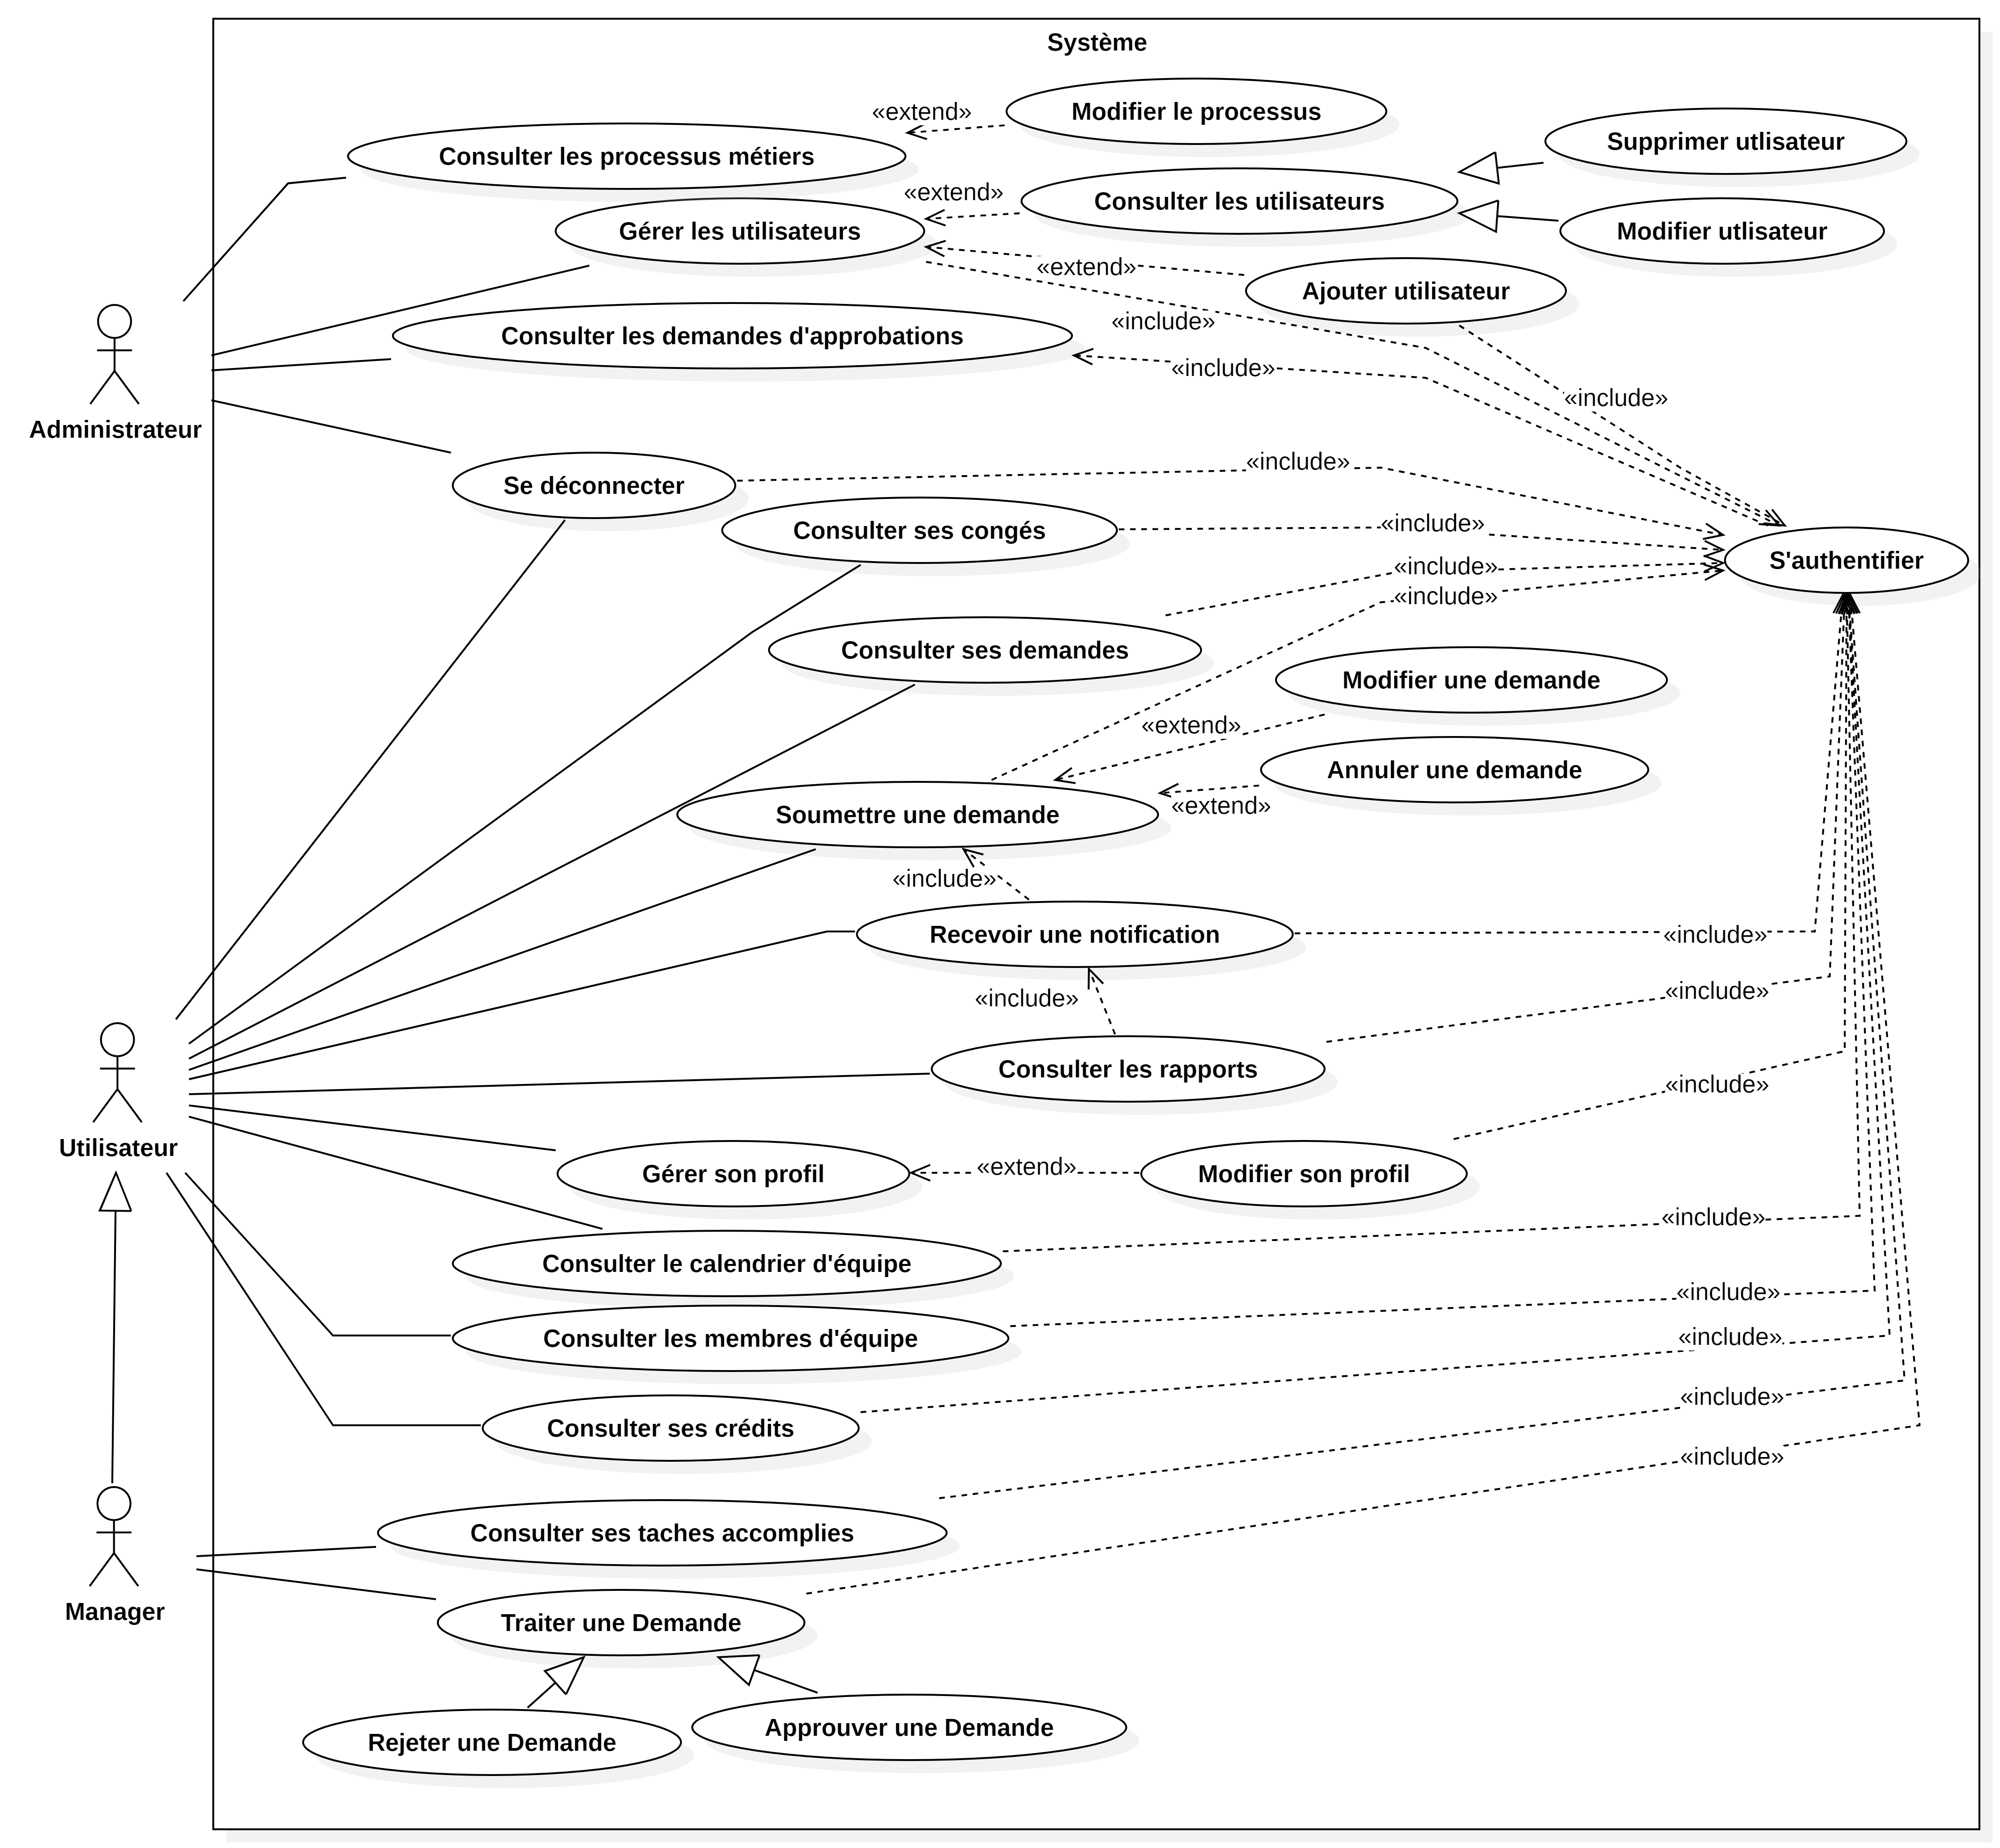
\includegraphics[width=20cm]{images/UseCaseDiagram.jpg}
\caption{Diagramme de cas d'utilisation globale}
\label{usecaseDiagram}
\end{adjustwidth}
\end{figure}
\newpage
\section{Diagramme de classe global}
Le diagramme de classe globale illustré dans la figure \ref{classDiagram} montre la constitution du système
à l’aide de la modélisation de ses classes, ses attributs, ses opérations et l’identification
des relations entre ses objets.
\begin{figure}[H]
\begin{adjustwidth}{-2cm}{-2cm} % reduce left and right margins locally
\centering
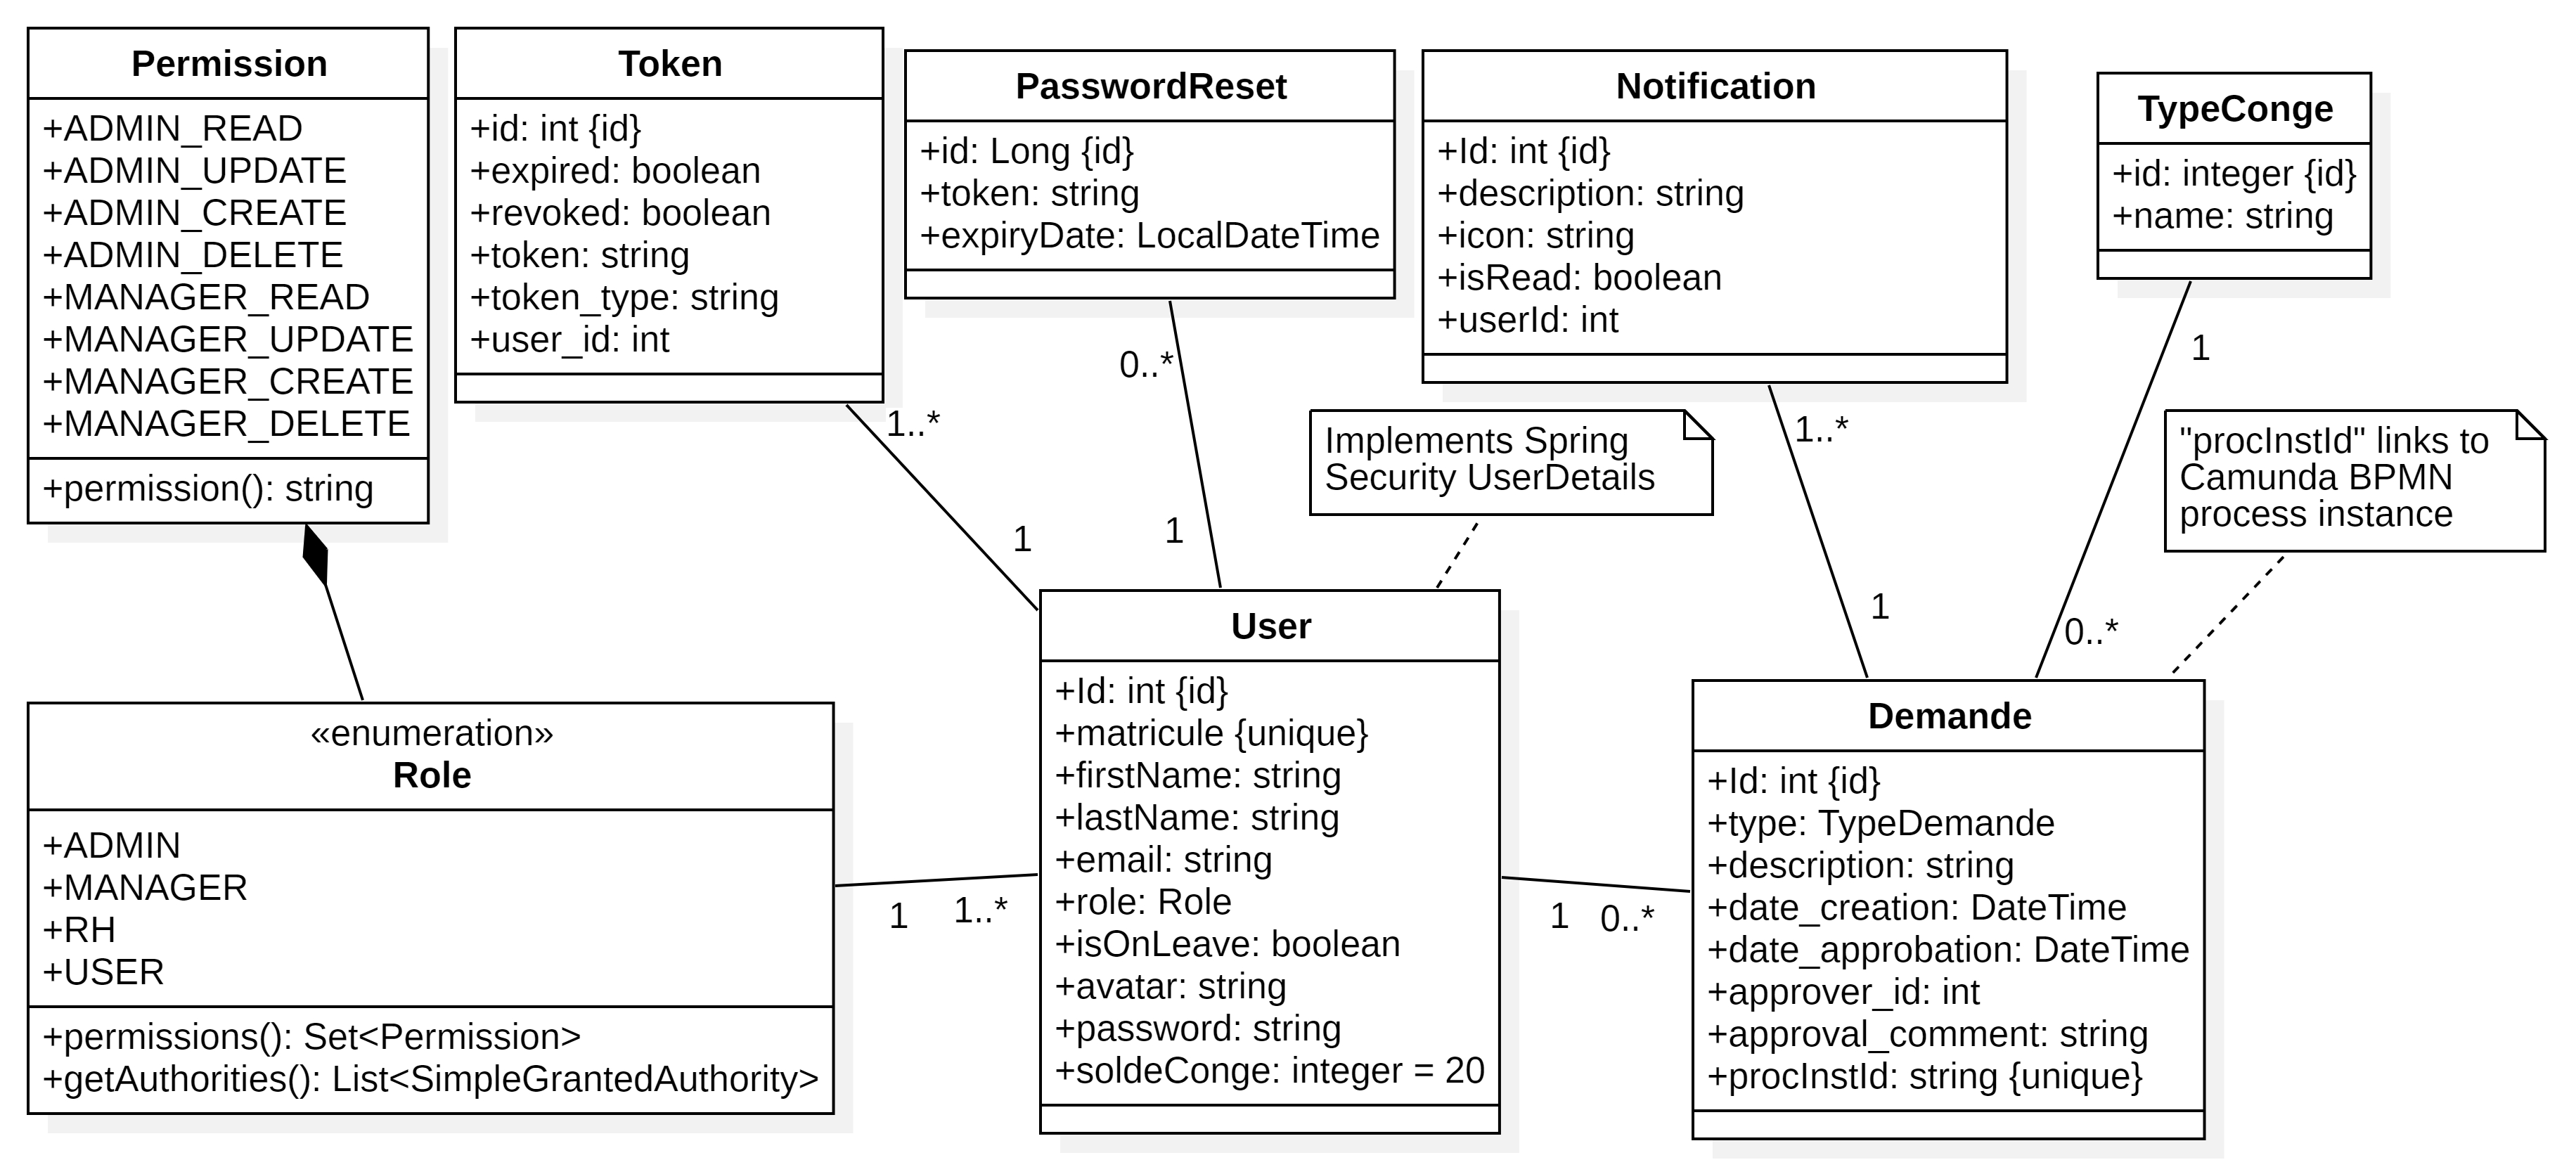
\includegraphics[width=21cm]{images/ClassDiagram.jpg}
\caption{Diagramme de classe globale}
\label{classDiagram}
\end{adjustwidth}
\end{figure}
\section{Backlog du Produit}
Le backlog du produit est un ensemble de tâches priorisées qui caractérise un produit. C'est l'un des éléments indispensables de la méthodologie Scrum. C'est l’outil de travail du Product Owner.\\
Ce qui nous mène à le modéliser dans le tableau \ref{tab:backlog_part1} et \ref{tab:backlog_part2} \cite{}:
\newpage
\begin{table}[h!]
\vspace*{-1.5cm}
\begin{adjustwidth}{-3cm}{-2.7cm}
\centering
\renewcommand{\arraystretch}{1.1}
\begin{tabular}{|p{0.18\textwidth}|p{0.24\textwidth}|p{0.40\textwidth}|p{0.08\textwidth}|}
\hline
\textbf{Sprint} & \textbf{User Story} & \textbf{Description} & \textbf{Priorité} \\
\hline
\multirow{4}{*}{\parbox{0.18\textwidth}{\raggedright Sprint 1 : Accès et Administration de Base}} 
    & \textbullet\ S'authentifier & \textbullet\ \raggedright Permet à tous les utilisateurs d’accéder à la plateforme via nom d’utilisateur et mot de passe. & 1 \\
    & \textbullet\ Se déconnecter & \textbullet\ \raggedright Permet aux utilisateurs de quitter le système après vérification des coordonnées. & 1 \\
    & \textbullet\ Gérer les utilisateurs & \textbullet\ \raggedright L’Administrateur peut ajouter, consulter, modifier et supprimer des utilisateurs. & 1 \\
    & \textbullet\ Mise en place et configuration de Camunda & \textbullet\ \raggedright Permet de configurer et d’intégrer le moteur Camunda dans l’application Spring Boot pour orchestrer les processus métiers. & 1 \\
\hline
\multirow{6}{*}{\parbox{0.18\textwidth}{\raggedright Sprint 2 : Gestion des Demandes}} 
    & \textbullet\ Gérer son profil & \textbullet\ \raggedright Chaque acteur modifie ses informations personnelles (mot de passe, e-mail, etc.). & 2 \\
    & \textbullet\ Réinitialiser son mot de passe & \textbullet\ \raggedright En cas d’oubli, l’utilisateur peut réinitialiser son mot de passe via un lien sécurisé. & 2 \\
    & \textbullet\ Soumettre une demande & \textbullet\ \raggedright Les Utilisateurs, Managers et RH soumettent des demandes (congés, absences, etc.). & 2 \\
    & \textbullet\ Consulter ses demandes & \textbullet\ \raggedright Les Utilisateurs, Managers et RH consultent l’historique de leurs demandes. & 2 \\
    & \textbullet\ Consulter ses congés & \textbullet\ \raggedright Les Utilisateurs, Managers et RH consultent leurs congés et leur solde. & 2 \\
    & \textbullet\ Traiter une demande & \textbullet\ \raggedright Les Managers et RH valident ou rejettent les demandes soumises. & 2 \\
\hline
\multirow{5}{*}{\parbox{0.18\textwidth}{\raggedright Sprint 3 : Suivi et Supervision}} 
    & \textbullet\ Recevoir une notification & \textbullet\ \raggedright Les Utilisateurs, Managers et RH reçoivent des alertes sur des actions importantes. & 2 \\
    & \textbullet\ Consulter les processus métiers & \textbullet\ \raggedright L’Administrateur consulte les processus métiers définis dans le système. & 3 \\
    & \textbullet\ Consulter les demandes d’approbation & \textbullet\ \raggedright L’Administrateur accède aux demandes soumises pour consultation. & 3 \\
    & \textbullet\ Consulter les membres de l’équipe & \textbullet\ \raggedright Les Utilisateurs, Managers et RH accèdent aux infos des membres de leur équipe. & 3 \\
    & \textbullet\ Consulter ses crédits & \textbullet\ \raggedright Les Utilisateurs, Managers et RH vérifient leur solde de congés ou crédits. & 2 \\
\hline
\end{tabular}
\caption{Backlog du Produit - Partie 1}
\label{tab:backlog_part1}
\end{adjustwidth}
\end{table}

\clearpage

\begin{table}[h!]
    \vspace*{-1.5cm}
    \begin{adjustwidth}{-3cm}{-2.7cm}
    \centering
    \renewcommand{\arraystretch}{1.1}
    \begin{tabular}{|p{0.18\textwidth}|p{0.24\textwidth}|p{0.40\textwidth}|p{0.08\textwidth}|}
    \hline
    \textbf{Sprint} & \textbf{User Story} & \textbf{Description} & \textbf{Priorité} \\
    \hline
    \multirow{5}{*}{\parbox{0.18\textwidth}{\raggedright Sprint 4 : Analyse et Améliorations}} 
        & \textbullet\ Consulter le calendrier d’équipe & \textbullet\ \raggedright Les Utilisateurs, Managers et RH consultent les absences et événements d’équipe. & 3 \\
        & \textbullet\ Consulter les tâches accomplies & \textbullet\ \raggedright Les Managers et RH suivent les tâches réalisées par leurs subordonnés. & 3 \\
        & \textbullet\ Consulter les rapports & \textbullet\ \raggedright Les Utilisateurs, Managers et RH consultent des rapports sur leurs activités. & 4 \\
        & \textbullet\ Exporter les rapports & \textbullet\ \raggedright Permet d’exporter les rapports (PDF, Excel) pour une utilisation hors ligne. & 4 \\
        & \textbullet\ Implémentation d’un chatbot & \textbullet\ \raggedright Permet de développer et d’intégrer un chatbot dans l’application pour assister les utilisateurs dans leurs interactions (consultation, soumission de demandes, etc.). & 4 \\
    \hline
    \multirow{6}{*}{\parbox{0.18\textwidth}{\raggedright Sprint 5 : Pipeline DevOps et Gestion GitOps}} 
        & \textbullet\ Installation Automatisée & \textbullet\ \raggedright Créer un playbook Ansible pour installer MicroK8s, ArgoCD et leurs dépendances, incluant les add-ons Ingress et DNS, pour un déploiement rapide et fiable et configurer ArgoCD pour synchroniser automatiquement avec le dépôt k8s-manifests et gérer les déploiements. & 4 \\
        & \textbullet\ Workflows CI & \textbullet\ \raggedright Implémenter des workflows GitHub Actions pour construire et pousser les images Docker vers DockerHub, avec mise à jour des tags dans k8s-manifests. & 5 \\
        & \textbullet\ Runner SonarQube & \textbullet\ \raggedright Configurer un runner auto-hébergé pour exécuter SonarScanner et analyser la qualité du code dans l’instance SonarQube locale. & 5 \\
        & \textbullet\ Gestion des Secrets & \textbullet\ \raggedright Encoder les variables sensibles (identifiants DB, tokens API) en Base64 et les gérer via des secrets Kubernetes. & 5 \\
        & \textbullet\ Exposition des Services & \textbullet\ \raggedright Déployer des règles Ingress pour exposer les services frontend, backend et SonarQube. & 6 \\
        & \textbullet\ Surveillance et Rollback & \textbullet\ \raggedright Vérifier la surveillance automatique des déploiements et le rollback natif d’ArgoCD en cas d’échec d’un nouveau pod. & 6 \\
    \hline
    \end{tabular}
    \caption{Backlog du Produit - Partie 2}
    \label{tab:backlog_part2}
    \end{adjustwidth}
    \end{table}
    \clearpage
\section{Planification de projet}
Cette section a pour objectif de présenter la planification de notre projet. Pour ce faire, nous utiliserons un diagramme de Gantt qui permettra de visualiser les différentes étapes du projet sous forme de tâches à réaliser, facilitant ainsi le suivi et l’organisation du travail.
\subsection{Diagramme de Gantt}
Le diagramme de Gantt présenté par la figure \ref{fig:diagantt} nous permet de visualiser les différentes tâches ainsi que leurs durées.

\begin{figure}[H]
\vspace*{-0.5cm}
     \centering
  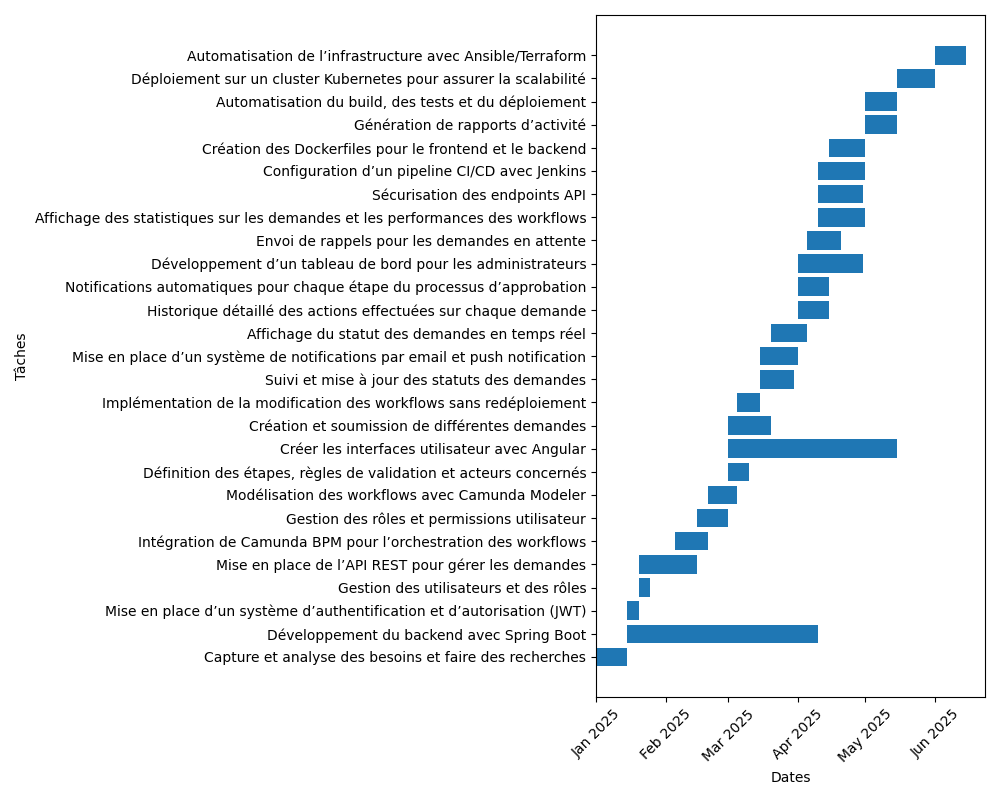
\includegraphics[scale=0.6]{images/gantt.png}
        \caption{Diagramme de Gantt} 
  \label{fig:diagantt}
 \end{figure}

%à ajouter le diagramme le Gantt 
\section{Environnement de travail}
Dans cette section, nous examinerons les différentes outils technologiques adoptées dans le cadre de ce projet.
\newpage
\subsection{Environnement materiel}
Durant ce projet,nous avons utilisé deux machines pour bien mener notre projet.Les caractéristiques techniques de ces machines sont présentés dans le tableau \ref{tab:specs}.

\begin{table}[h!]
\centering
\caption{Spécifications des machines utilisées}
\label{tab:specs}
\begin{tabularx}{\linewidth}{|X|X|X|}
\hline
\textbf{} & \textbf{Machine 1} & \textbf{Machine 2} \\
\hline
\textbf{Marque} & Gigabyte AERO 15 & Machine virtuelle \\
\hline
\textbf{Système d’exploitation} & Windows 11 64 bit & Ubuntu 22.04 64 bit \\
\hline
\textbf{Processeur} & I7-11800H 2.3 GHz & I5-11400F 2.6 GHz \\
\hline
\textbf{RAM} & 16 GB 3200MHz & 16 GB 3200MHz \\
\hline
\textbf{Disque Dur} & 1 TB & 500 GB \\
\hline
\end{tabularx}
\end{table}
\subsection{Environnement logiciel}
Dans cette section, nous présentons l’environnement logiciel utilisé dans ce projet :

\begin{itemize}
 \item \textbf{Git}Dont le logo est présenté dans la figure \ref{fig:git}, cet outil constitue un système de gestion de versions distribué. Il permet de tracer l’évolution des fichiers et des répertoires d’un projet, d’accéder à des versions précédentes et de consulter en détail l’historique des modifications réalisées.
 \begin{figure}[h]
    \centering
    
\includegraphics[width=2.5cm]{images/git.png}
    \caption{Logo de Git}
    \label{fig:git}
\end{figure}
\item \textbf{Github}:Dont le logo est exposé dans la figure \ref{fig:gituhbl}, 
 est une plateforme collaborative basée sur Git, utilisée pour héberger du code, suivre les changements et faciliter le travail d’équipe sur des projets de développement logiciel.
 \begin{figure}[h]
    \centering
    
\includegraphics[width=2.2cm]{images/githubl.png}
    \caption{Logo de Github}
    \label{fig:gituhbl}
\end{figure}
\item \textbf{WampServer}:Dont le logo est illustré dans la figure \ref{fig:wamp}, WampServer est un environnement de développement web local pour Windows. Il regroupe Apache, MySQL et PHP, permettant aux développeurs de tester et d’exécuter des applications web en local avant leur mise en production.
 \begin{figure}[h]
    \centering
    
\includegraphics[width=1.8cm]{images/WampServer.png}
    \caption{Logo de WampServer}
    \label{fig:wamp}
\end{figure}
\item \textbf{phpMyAdmin}:Dont le logo est représenté dans la figure \ref{fig:phpmyadmin}, phpMyAdmin est une interface web permettant d’administrer facilement des bases de données MySQL ou MariaDB. Il offre aux utilisateurs un accès simplifié pour gérer les tables, exécuter des requêtes SQL, importer ou exporter des données, le tout sans avoir à utiliser la ligne de commande.
 \begin{figure}[h]
    \centering
    
\includegraphics[width=2.9cm]{images/phpmyadmin.png}
    \caption{Logo de phpMyAdmin}
    \label{fig:phpmyadmin}
\end{figure}
\item \textbf{Visual Studio Code (VSCode)}:Représenté dans la figure \ref{fig:vscode}, VSCode est un éditeur de code source léger et extensible, populaire pour le développement Angular. Il offre une riche palette d’extensions, telles que des outils de linting, de débogage, et des intégrations Git, ce qui le rend idéal pour travailler sur des applications JavaScript et TypeScript, comme celles développées avec Angular.
 \begin{figure}[h]
    \centering
    
\includegraphics[width=1.6cm]{images/vscode.png}
    \caption{Logo de VSCode}
    \label{fig:vscode}
\end{figure}
\item \textbf{IntelliJ IDEA}:Représenté dans la figure \ref{fig:intellij}, IntelliJ IDEA est un environnement de développement intégré (IDE) robuste, principalement utilisé pour le développement d'applications Java, telles que celles créées avec Spring. Il offre des fonctionnalités avancées comme la gestion des dépendances, le débogage intégré, et la prise en charge complète de Spring, ce qui facilite le développement et le déploiement d’applications Spring Boot.
 \begin{figure}[h]
    \centering
    
\includegraphics[width=1.8cm]{images/intellij.png}
    \caption{Logo de IntelliJ}
    \label{fig:intellij}
\end{figure}
\newpage
\end{itemize}
\section{Choix technologiques}
\begin{itemize}
 \subsection{Frontend}
\item \textbf{Angular}:Représenté dans la figure \ref{fig:angular}, Angular est un framework de développement web permettant de créer des applications web dynamiques et interactives.
 \begin{figure}[h]
    \centering
    
\includegraphics[width=1.8cm]{images/angular.png}
    \caption{Logo d'Angular}
    \label{fig:angular}
\end{figure}
 \subsection{Backend}
\item \textbf{Spring Boot}:Représenté dans la figure \ref{fig:SpringBoot}, Spring Boot est un framework Java qui facilite le développement d’applications Spring en simplifiant la configuration et le déploiement, tout en offrant des outils prêts à l’emploi comme un serveur embarqué et une sécurité intégrée.
 \begin{figure}[h]
    \centering
    
\includegraphics[width=1.6cm]{images/SpringBoot.png}
    \caption{Logo de Spring Boot}
    \label{fig:SpringBoot}
\end{figure}
\subsection{Workflow}
\item \textbf{Camunda}:Dont le logo est représenté dans la figure \ref{fig:camunda}, Camunda est une plateforme open-source de gestion des processus métier (BPMN), de gestion des décisions (DMN) et de gestion des cas (CMMN). Camunda est particulièrement utilisé pour l'orchestration des workflows complexes et s'intègre facilement dans des architectures Java et microservices.
 \begin{figure}[h]
    \centering
    
\includegraphics[width=1.6cm]{images/camunda.png}
    \caption{Logo de Camunda}
    \label{fig:camunda}
\end{figure}
\newpage
\subsection{Base de données}
\item \textbf{MySQL}:Représenté dans la figure \ref{fig:MySQL}, MySQL est un système de gestion de bases de données relationnelles open-source. Il permet de stocker, gérer et interroger des données de manière structurée à l'aide de SQL.
 \begin{figure}[h]
    \centering
    
\includegraphics[width=2.3cm]{images/MySQL.png}
    \caption{Logo de MySQL}
    \label{fig:MySQL}
\end{figure}
\subsection{CI/CD}
\item \textbf{ArgoCD}:Représenté dans la figure \ref{fig:ArgoCD}, ArgoCD est un outil open-source d'intégration et de déploiement continu (CI/CD) spécialement conçu pour Kubernetes. Il permet de déployer et gérer des applications dans des environnements Kubernetes en suivant la méthodologie GitOps.
 \begin{figure}[h]
    \centering
    
\includegraphics[width=1.6cm]{images/ArgoCD.png}
    \caption{Logo d'ArgoCD}
    \label{fig:ArgoCD}
\end{figure}
\subsection{Conteneurisation}
\item \textbf{Docker}:Représenté dans la figure \ref{fig:docker}, Docker est une plateforme open-source permettant de créer, déployer et exécuter des applications dans des conteneurs. Ces conteneurs encapsulent l’application et ses dépendances dans un environnement léger et portable.
 \begin{figure}[h]
    \centering
    
\includegraphics[width=2.5cm]{images/docker.png}
    \caption{Logo de Docker}
    \label{fig:docker}
\end{figure}
\newpage
\subsection{Orchestration}
\item \textbf{Kubernetes}:Représenté dans la figure \ref{fig:kubernetes}, Kubernetes est un système open-source d'orchestration de conteneurs qui automatise le déploiement, la gestion, la mise à l’échelle et l’administration des applications conteneurisées. Il permet de gérer efficacement les clusters de conteneurs Docker, offrant des fonctionnalités telles que l’autoscaling, la gestion des ressources et le monitoring des applications.
 \begin{figure}[h]
    \centering
    
\includegraphics[width=1.6cm]{images/kubernetes.png}
    \caption{Logo de Kubernetes}
    \label{fig:kubernetes}
\end{figure}
\end{itemize}
\section*{Conclusion}
Dans ce deuxième chapitre, nous avons détaillé les besoins fonctionnels et non fonctionnels du projet, ainsi que les différents acteurs et leurs interactions avec le système à travers des diagrammes de cas d'utilisation et de classes globaux. Nous avons également présenté le backlog du produit, structuré en sprints, et défini les priorités pour chaque fonctionnalité.
Nous avons également présenté les choix technologiques retenus pour le développement du projet, couvrant l'environnement matériel, l'environnement logiciel.
Le chapitre suivant sera consacré à la présentation du Sprint 1, qui couvrira les premières étapes du développement, notamment l'accès et l'administration de base du système.



